% ****** Start of file apssamp.tex ******
%
%   This file is part of the APS files in the REVTeX 4.1 distribution.
%   Version 4.1r of REVTeX, August 2010
%
%   Copyright (c) 2009, 2010 The American Physical Society.
%
%   See the REVTeX 4 README file for restrictions and more information.
%
% TeX'ing this file requires that you have AMS-LaTeX 2.0 installed
% as well as the rest of the prerequisites for REVTeX 4.1
%
% See the REVTeX 4 README file
% It also requires running BibTeX. The commands are as follows:
%
%  1)  latex apssamp.tex
%  2)  bibtex apssamp
%  3)  latex apssamp.tex
%  4)  latex apssamp.tex
%
\documentclass[%
 reprint,
nofootinbib,
%superscriptaddress,
%groupedaddress,
%unsortedaddress,
%runinaddress,
%frontmatterverbose,
%preprint,
%showpacs,preprintnumbers,
%nofootinbib,
%nobibnotes,
%bibnotes,
aps,
%pra,
%prb,
%rmp,
%prstab,
%prstper,
%floatfix,
]{revtex4-1}

\usepackage[utf8]{inputenc}
\usepackage[english]{babel}
\usepackage{dsfont}
\usepackage{amsmath}
\usepackage{amssymb}
\usepackage{graphicx}% Include figure files
\usepackage{dcolumn}% Align table columns on decimal point
\usepackage{bm}% bold math
\usepackage{amsmath}
\usepackage{varioref}
\usepackage{booktabs}
\usepackage[bottom]{footmisc}

\usepackage{wasysym}

\usepackage{physics}

\usepackage{algpseudocode}
\usepackage{listings}

\usepackage{booktabs}

\usepackage{tikz}

\newcommand{\RN}[1]{%
  \textup{\uppercase\expandafter{\romannumeral#1}}%
}


\newcolumntype{C}{>{$}c<{$}}
\AtBeginDocument{
\heavyrulewidth=.08em
\lightrulewidth=.05em
\cmidrulewidth=.03em
\belowrulesep=.65ex
\belowbottomsep=0pt
\aboverulesep=.4ex
\abovetopsep=0pt
\cmidrulesep=\doublerulesep
\cmidrulekern=.5em
\defaultaddspace=.5em
}

%\usepackage{hyperref}% add hypertext capabilities
%\usepackage[mathlines]{lineno}% Enable numbering of text and display math
%\linenumbers\relax % Commence numbering lines

%\usepackage[showframe,%Uncomment any one of the following lines to test
%%scale=0.7, marginratio={1:1, 2:3}, ignoreall,% default settings
%%text={7in,10in},centering,
%%margin=1.5in,
%%total={6.5in,8.75in}, top=1.2in, left=0.9in, includefoot,
%%height=10in,a5paper,hmargin={3cm,0.8in},
%]{geometry}

\begin{document}

%\preprint{APS/123-QED}

\title{Phase transitions in 2D Ising ferromagnets}% Force line breaks with \\

\author{Cecilie Glittum}\homepage{http://www.github.uio.no/cecilgl/FYS4150}

\affiliation{%
 Department of Physics, University of Oslo\\
}%


\date{\today}% It is always \today, today,
             %  but any date may be explicitly specified

\begin{abstract}
A numerical study of phase transitions in an Ising ferromagnet on a two dimensional square lattice done in collaboration with Ivar Svalheim Haugerud. We use Monte Carlo simulations with the Metropolis algorithm to find the critical temperature of a 2D Ising ferromagnet with periodic boundary conditions. We benchmark by using analytical results for a $2\times 2$ lattice. By studying a $20\times 20$ lattice we find that an equilibration time of $10^4$ Monte Carlo cycles is needed to reach steady state. For the same system, we also study the probability distribution function. Compared to the variance for high temperatures, the variance for low temperatures is small. We parallelize our code using MPI in order to be able to study bigger systems. By using four CPUs we're able to make the run time $3.6(2)$ times faster. We then study larger systems. By applying a Savitzky-Golay filter to the measured heat capacities and doing a linear regression, we extract the critical temperature for an infinite lattice size to be $T_C(L\to\infty) = 2.2698(6) J/k_B$.
\end{abstract}


\maketitle


\section{Introduction}

Magnetism is an active area of research, due to its many applications in e.g. technology and industry. Magnetism is also believed to play a role in the understanding of important materials like high temperature superconductors.

There exists several classes of magnets, where the ferromagnetic magnets are the most studied. Ferromagnetic materials have interacting microscopic magnetic moments that tend to align in the same direction at low temperatures. By increasing the temperature, the spins begin to fluctuate, and at a temperature $T_C$ they go from being in an ordered phase to an disordered phase. This is known as a phase transition.

We study here the Ising model with ferromagnetic interactions. It is a simplified classical model of ferromagnetic materials that only take the $z$-component of the spins into account. Our study is even more specified to the case of spins on a two dimensional square lattice. We look at nearest-neighbour interactions, and neglect all other interactions.

The Ising model on an infinite square lattice was solved analytically by L. Onsager in 1944. He found the critical temperature to be $k_BT_C/J = 2.2692$ \citep{onsager}. We try here to reproduce the result of L. Onsager by Monte Carlo (MC) simulations on finite sized systems. The Monte Carlo algortihm is based on Markov chains, which ensures that the configuration of our system converges towards the equilibrium configuration if the number of MC cycles go to infinity. We use the Metropolis algorithm as accepting rule.

In our simulations, we will start by benchmarking our implementation against analytical expressions for a $2\times 2$ lattice. We then increace the latticce size to $20 \times 20$ to study the equilibration time of our MC algorithm. We also study how frequent the proposed states are accepted and study the energy distribution. Afterwards we try to localize the critical temperature of the 2D Ising ferromagnet on a square lattice for different lattice sizes, which can be used to estimate the critical temperature in the limit of an infinite lattice. 

In this article, we first look at the theory of the Ising model and phase transitions in magnetic materials, we proceed by studying the Monte Carlo algorithm used to find the steady state configuration of the system. We then present the results of our simulations followed by a discussion and conclusion.

\section{Theory}

\subsection{The Ising model}

The Ising model is a model of magnetism in which spins of unit length are only allowed to point up or down, i.e. we only consider the $z$-component of the spins. 

The Hamiltonian of the  two dimensional Ising model is
\begin{equation}\label{eq:Hamiltonian}
H = -J\sum_{\langle ij \rangle}S^z_i S^z_j,
\end{equation}
where $\langle ij \rangle$ denotes a sum over the nearest neighbours of each spin. $J$ is the coupling constant that determines the interaction between the spins. If $J$ is positive(negative), we have (anti)ferromagnetic interactions between the spins, which means that the spins tends to (anti)align. Thus, we will take $J$ to be positive.

The 2D Ising model on an infinite square lattice is solved analytically, by L. Onsager \cite{onsager}. He found the critical temperature to be
\begin{equation}
k_B T_C / J = \frac{2}{\ln (1 + \sqrt{2})} \approx 2.2692.
\end{equation}



\subsection{Analytical expressions for a $\boldsymbol{2 \times 2}$ lattice}

We must look at a small system to be able to calculate e.g. the  partition function, which is needed to get analytical expressions for physical quantities like the susceptibility and heat capacity. For a $2 \times 2$ lattice with periodic boundary conditions, the possible energies and magnetizations are stated together with degeneracies in Table \ref{table:2times2}. 

% Please add the following required packages to your document preamble:
% \usepackage{booktabs}
\begin{table}[]
\caption{The number of spins pointing up on a $2\times 2$ lattice with corresponding degeneracies, energies and magnetizations. The energies are calculated with periodic boundary conditions.}
\label{table:2times2}
\begin{tabular}{@{}cccc@{}}
\toprule
$\quad$\#spins$\quad$ & deg. & $E [J]$   & $M$  \\ \midrule
$4$     & $\qquad 1\qquad$  & $\quad-8\quad$ & $4$  \\
$3$     & $4$  & $0$   & $2$  \\
$2$     & $4$  & $0$   & $0$  \\
$2$     & $2$  & $+8$ & $0$  \\
$1$     & $4$  & $0$   & $-2$ \\
$0$     & $1$  & $-8$ & $\qquad -4\qquad$ \\ \bottomrule
\end{tabular}
\end{table}

The energy is calculated from Eq. \eqref{eq:Hamiltonian}, while the magnetization is the sum of all the spins,
\begin{equation}
M = \sum_{i = 1}^{N} S^z_i,
\end{equation}
where $N$ is the total number of spins.

By using Table \ref{table:2times2}, we can calculate the mean energy $\ev{E}$, mean energy squared $\ev{E^2}$, mean (absolute) magnetization $\ev{\abs{M}}$ and mean magnetization squared $\ev{M^2}$. We have that the thermal average of a physical quantity is given by
\begin{equation}
\ev{A} = \frac{1}{Z} \sum_i A_i e^{-\beta E_i},
\end{equation}
where $i$ runs over all micro states, $\beta = 1/k_B T$ and $Z$ is the partition function, which in the $2 \times 2$ case is
\begin{equation}
Z = \sum_i e^{-\beta E_i} = 4\left(3 + \cosh (8\beta J)\right).
\end{equation}

We then get
\begin{align}\label{eq:expvals}
\ev{E} &= \frac{1}{Z} \sum_i E_i e^{-\beta E_i} = -\frac{1}{Z}32J\sinh (8\beta J),\\
\ev{E^2} &= \frac{1}{Z} \sum_i E_i^2 e^{-\beta E_i} = \frac{1}{Z}256J^2\cosh (8\beta J),\\
\ev{\abs{M}} &= \frac{1}{Z} \sum_i \abs{M_i} e^{-\beta E_i} = \frac{1}{Z}8\left(2 + e^{8\beta J}\right),\\
\ev{M^2} &= \frac{1}{Z} \sum_i M_i^2 e^{-\beta E_i} = \frac{1}{Z}32\left( 1 + e^{8\beta J}\right).
\end{align}

From these expectation values, we can calculate the heat capacity at constant volume and the susceptibility of the system from the following relations \cite{hjorten}:
\begin{equation}\label{eq:heatcap}
C_V(T) = \frac{1}{k_BT^2}\left(\ev{E(T)^2} - \ev{E(T)}^2\right),
\end{equation}
\begin{equation}\label{eq:suscept}
\chi(T) = \frac{1}{k_B T}\left(\ev{M(T)^2} - \ev{M(T)}^2\right).
\end{equation}



\subsection{Phase transitions in magnetic systems}

For the Ising ferromagnet, there is a phase transition from the unordered paramagnetic state to the ordered ferromagnetic state. This happens when the temperature falls below the so-called critical temperature $T_C$, where the magnetic couplings between the spins outperform the thermal fluctuations of the spins.

For a system like an 2D Ising ferromagnet, the Helmholtz free energy must be minimized to reach an equilibrium state. This is a fight between the minimization of the average energy and the maximization of the entropy, as the minimal energy state for a ferromagnet obviously is the ordered state where all spins align, which is also the state of minimal entropy.


In the vicinity of the critical temperature, many physical quantities are characterized by a power-law behaviour. As an example, for the Ising class of models, the mean magnetization is given by
\begin{equation}
\ev{M(T)} \sim (T - T_C)^\beta,
\end{equation}
where $\beta = 1/8$ is a so-called critical exponent. A similar relation applies to the heat capacity
\begin{equation}
C_V(T) \sim \abs{T_C - T}^{-\alpha},
\end{equation}
and the susceptibility
\begin{equation}
\chi (T) \sim \abs{T_C -T}^{-\gamma},
\end{equation}
with the critical exponents $\alpha = 0$ and $\gamma = 7/4$ \cite{flekkoy, hjorten}.

The correlation length $\xi$ is expected to be of the order of the lattice spacing for $T \gg T_C$; That is, there is no correlation between the spins at temperatures much higher than the critical temperature. This is easily understood by the fact that we are in the disordered phase where the thermal fluctuations outclass the magnetic interactions. As $T$ approaches $T_C$ from the disordered phase, the spins become more and more correlated, thus the correlation length increases. The divergent behaviour at the phase transition is
\begin{equation}\label{eq:nu}
\xi (T) = \abs{T_C - T}^{-\nu}.
\end{equation}
A continuous phase transition is characterized by a correlation length that spans the whole system \cite{hjorten}. Through so-called finite size scaling relations it is possible to relate the behaviour at finite lattices with the results for an infinitely large lattice. The critical temperature then scales as
\begin{equation}\label{eq:TCinfty}
T_C(L) - T_C(L = \infty) = aL^{-1/\nu},
\end{equation}
where $a$ is a constant, and $\nu$ is defined in Eq. \eqref{eq:nu}. We can then obtain
\begin{align}
\ev{M(T)} &\sim (T - T_C)^\beta \rightarrow L^{-\beta/\nu},\\
C_V(T) &\sim \abs{T - T_C}^{-\alpha} \rightarrow L^{\alpha/\nu},\\
\chi (T) &\sim \abs{T - T_C}^{-\gamma} \rightarrow L^{\gamma/\nu}.
\end{align}
We see from these relations that the heat capacity and the susceptibility should diverge at the phase transition.

The mean magnetization should be zero above $T_C$ and non-zero below $T_C$, thus this serves as our order parameter.


\section{Algorithms}

We simulate the 2D Ising model on a square lattice using Monte Carlo methods. For each Monte Carlo cycle, we sweep through the whole lattice and try to change the micro state of the system by flipping spins. The Metropolis algorithm dictates whether the new state is accepted or not.

\subsection{Monte Carlo simulations}

The principle of the Monte Carlo (MC) simulations is based on Markov chains, where the system evolves over time by multiplications of a stochastic matrix, and converges towards the most likely state.

The MC simulations use a probability distribution, and in the case of the canonical ensemble, we use Boltzmann statistics. Thus, to find all the probabilities, we need to calculate the partition function, which is overwhelming when the number of lattice points increase, due to an enormous number of possible states. By using MC simulations with the Metropolis algorithm, we avoid this problem as the Metropolis algorithm only considers the ratios between probabilities. Thus, the partition function cancels, and we only have to calculate the Boltzmann factors.

In our MC simulations, we create a random initial state, where the spins have an equal probability of pointing up or down. Then, for each MC cycle, we sweep through the lattice randomly, trying to flip a spin $L^2$ times. Each time we try to flip a spin, we call the Metropolis algorithm to see if the new configuration is accepted or not.

\subsubsection{The Metropolis algorithm}

The Metropolis algorithm is the accepting rule we use in our Monte Carlo simulations. It calculates the change in energy after one spin is flipped $\Delta E$ as
\begin{equation}
\Delta E = 2JS^1_l\sum_{\langle k \rangle}S_k,
\end{equation}
where $S^1_l$ is the value of the spin \textit{before} it gets flipped and $S_k$ are the neighbouring spins. As we only consider nearest neighbour interactions, there are only five different possible values for $\Delta E$ when one spin is flipped. These are listed in Table \ref{table:DeltaE}. Because there are only five possibilities of $\Delta E$, the factor $e^{-\beta\Delta E}$ used by the Metropolis algorithm can be precalculated for each temperature, so that a lot of FLOPS are spared by not doing excessive calls to the exponential function.

% Please add the following required packages to your document preamble:
% \usepackage{booktabs}
\begin{table}[]
\caption{The possible changes in energy $\Delta E$ when one spin is flipped. We see there only are five different possibilities for the two dimensional square lattice. Because we only consider nearest-neighbour interactions, the change in energy is only dependent on the configurations of the nearest neighbours in relation to the spin we're flipping.}
\label{table:DeltaE}
\begin{tabular}{@{}ccc|c@{}}
\toprule
$\quad$ Initial conf. $\quad$ &  & $\quad$ Final conf. $\quad$ & $\quad \Delta E [J] \quad$ \\ \midrule
$\begin{matrix}& \uparrow & \\ \uparrow & \uparrow & \uparrow \\ & \uparrow & \\ & & & \end{matrix}$ & $\quad \boldsymbol{\rightarrow} \quad$ & $\begin{matrix}& \uparrow & \\ \uparrow & \downarrow & \uparrow \\ & \uparrow & \\ & & & \end{matrix}$ & $8$ \\
$\begin{matrix}& \downarrow & \\ \uparrow & \uparrow & \uparrow \\ & \uparrow & \\ & & & \end{matrix}$ & $\boldsymbol{\rightarrow}$ & $\begin{matrix}& \downarrow & \\ \uparrow & \downarrow & \uparrow \\ & \uparrow & \\ & & & \end{matrix}$ & $4$ \\
$\begin{matrix}& \downarrow & \\ \downarrow & \uparrow & \uparrow \\ & \uparrow & \\ & & & \end{matrix}$ & $\boldsymbol{\rightarrow}$ & $\begin{matrix}& \downarrow & \\ \downarrow & \downarrow & \uparrow \\ & \uparrow & \\ & & & \end{matrix}$ & $0$ \\
$\begin{matrix}& \downarrow & \\ \downarrow & \uparrow & \downarrow \\ & \uparrow & \\ & & & \end{matrix}$ & $\boldsymbol{\rightarrow}$ & $\begin{matrix}& \downarrow & \\ \downarrow & \downarrow & \downarrow \\ & \uparrow & \\ & & & \end{matrix}$ & $-4$ \\
$\begin{matrix}& \downarrow & \\ \downarrow & \uparrow & \downarrow \\ & \downarrow & \\ & & & \end{matrix}$ & $\boldsymbol{\rightarrow}$ & $\begin{matrix}& \downarrow & \\ \downarrow & \downarrow & \downarrow \\ & \downarrow & \\ & & & \end{matrix}$ & $-8$ \\ \bottomrule
\end{tabular}
\end{table}

The Metropolis algorithm accepts the new micro state if 
\begin{itemize}
\item $\Delta E < 0$
\item $\Delta E > 0$ and $e^{-\beta \Delta E} \geq r$, where $r$ is a random number between $0$ and $1$.
\end{itemize}


If the new configuration is accepted, the current value for the energy and magnetization of the system is updated. After $L^2$ random spins are flipped, we update the expectation values for $E$, $E^2$, $M$, $M^2$ and $\abs{M}$, before the next MC cycle repeats.

Some important aspects of the Metropolis algorithm is that it fulfils both ergodicity and detailed balance, which are conditions needed for convergence towards the equilibrium state of the system.



As it takes some time for the configuration to converge towards equilibrium, the results should get better the more MC cycles that is used.



\section{Methods}

\subsection{Units}

We set $J = 1$ and $k_B = 1$ in our simulations. For dimensionless spins that equal $\pm 1$, the unit of energy will be $J$ and the unit of temperature will be $J/k_B$. Correspondingly, the magnetization is unitless, while the heat capacity has units of $k_B$ and the susceptibility has units of $1/J$.



\subsection{Random numbers}

The Monte Carlo algorithm requires a random number generator. It is important that the period of this generator is long enough so that it not starts repeating. At most we use $L = 200$ (where $L$ is the \textit{lattice size}, i.e. we have an $L \times L$ lattice) for $10^6$ MC cycles, which means that we generate $8\cdot 10^{10}$ random numbers. Thus, the period of our random number generator must be larger than this. The random number generator we have chosen to use is the Mersenne Twister random number generator, which has a period of $2^{19937}$.


\subsection{Boundary conditions}

Compared to actual physical systems, the systems in our simulations are small in size. To minimize boundary effects, we will impose periodic boundary conditions, so that our lattice effectively has the topology of a torus. 

When implementing this in our code, we take care of the periodic boundary conditions by including an index vector $[L-1, 0, 1, ..., L, L+1]$, so that the neighbours of  spin $0$ are spin $L-1$ and spin $1$ (in the 1D case). This index vectors is used in both dimensions, and ensures that all the spins have four neighbours. 

By using this index vector as index every time we use the matrix that stores the spins, we get periodic boundary conditions without any if-tests.


\subsection{Initial configurations}

When starting a new simulation we will always use a random initial configuration, even though the equilibration time may be smaller if we start in an ordered state for low temperatures.

When doing subsequent simulations for a range of temperatures, we will let the initial configuration be the equilibrium configuration of the preceding temperature. This should minimize the equilibration time if the two temperatures are close to each other, as the steady states are expected to look very much the same.



\subsection{Equilibration}

To get the most accurate results, we should wait with the calculation of expectation values after the system is in equilibrium. The initial configuration is in general not in equilibrium, and thus we want to equilibrate the system before we begin computing the various expectation values.

This can be done by manually looking at the data after the run and choose how many of the first MC cycles that should be excluded from the calculations. 

Another way to equilibrate is to choose a number of MC cycles to run without calculating the expectation values, then using the resulting state as initial state for the actual run. This is the method we will be using when trying to extract the critical temperature.

We will always equilibrate for a longer time for the first temperature than for the rest, as the first temperature in general is further away from equilibrium.


\subsection{Simulations}

We check our implementation by running the code for $L = 2$, as we know the analytical solutions in this case. 

We then run simulations for $L = 20$ to study how many Monte Carlo cycles is needed to reach the equilibrium state. We will use this to decide how many cycles we should use when equilibrating the system for each temperature, as it is first after equilibrium is reached that we want to start computing various expectation values. For the temperatures $T = 1.0J/k_B$ and $T = 2.4J/k_B$, we studied the mean energy and magnetization as functions of the number of MC cycles. We let the initial configuration be both random and ordered for both temperatures.

Thereafter we computed the probability distribution of energies $P(E)$ for both the temperatures ($L = 20$). We did this by counting the number of times a given energy appeared in the computations after equilibrium was reached. 

The main purpose of this study was to look at the behaviour of 2D Ising ferromagnets on a square lattice close to the critical temperature as a function of the lattice size. We therefore used Monte Carlo simulations with the Metropolis algorithm to calculate $\ev{E}$, $\ev{\abs{M}}$, $C_V$ and $\chi$ as functions of temperature for $L = 40, 60, 80, 100, 120, 200$ and temperatures in $T \in [2.02, 2.49]$. In general, we used a temperature step of $0.01J/k_B$, but we decreased it to $0.0025J/k_B$ close to the theoretical value of the critical temperature.

 A Savitzky-Golay filter was applied to the computed values for the heat capacity to smooth out the graph to minimize disturbance from fluctuations around the peak in the heat capacity. We used a seventh order polynomial with $47$ coefficients. The approximated critical temperature for a given $L$ was then taken to be the temperature where the filtered susceptibility has it maximum. This data was then analysed using Eq. \eqref{eq:TCinfty}, which tells us that for $\nu = 1$, we have a linear relation between the critical temperatures at different lattice sizes and $1/L$. By linear regression, we extracted $T_C(L\to\infty)$ as the intercept with the temperature axis.

We also wanted to study the evolution of the spin configurations above and below the critical temperature, and did so for a lattice of size $L = 1000$ for $T = 1.0J/k_B$ and $T = 2.4J/k_B$.


\subsection{Parallelization}

When doing MC simulations we are greedy, the more data, the better. Thus, our simulations take a lot of time, especially when studying large systems. Therefore, it is convenient to paralellize the code, so that we can take advantage of all the CPUs on the machine. We parallelize our code using MPI, and distribute the different temperatures we run for between the different CPUs. We let each CPU have a ``continuous'' range of temperatures, so that the previous equilibrium state works as initial state for the next temperature.

We also perform a timing analysis of some selected runs in order to see that we get an optimal speed up when parallelizing the code.

\section{Results}

\subsection{Benchmarking}
Fig. \vref{fig:taskb} shows the results of the Monte Carlo simulations for the $L = 2$ lattice for different temperatures. The results are plotted togehter with the analytical solutions given in Eqs. \eqref{eq:expvals} - \eqref{eq:suscept}. We used $10^6$ MC cycles, even though it looked like $10^5$ MC cycles would be sufficient for the $2 \times 2$ lattice.

\begin{figure*}
\centering
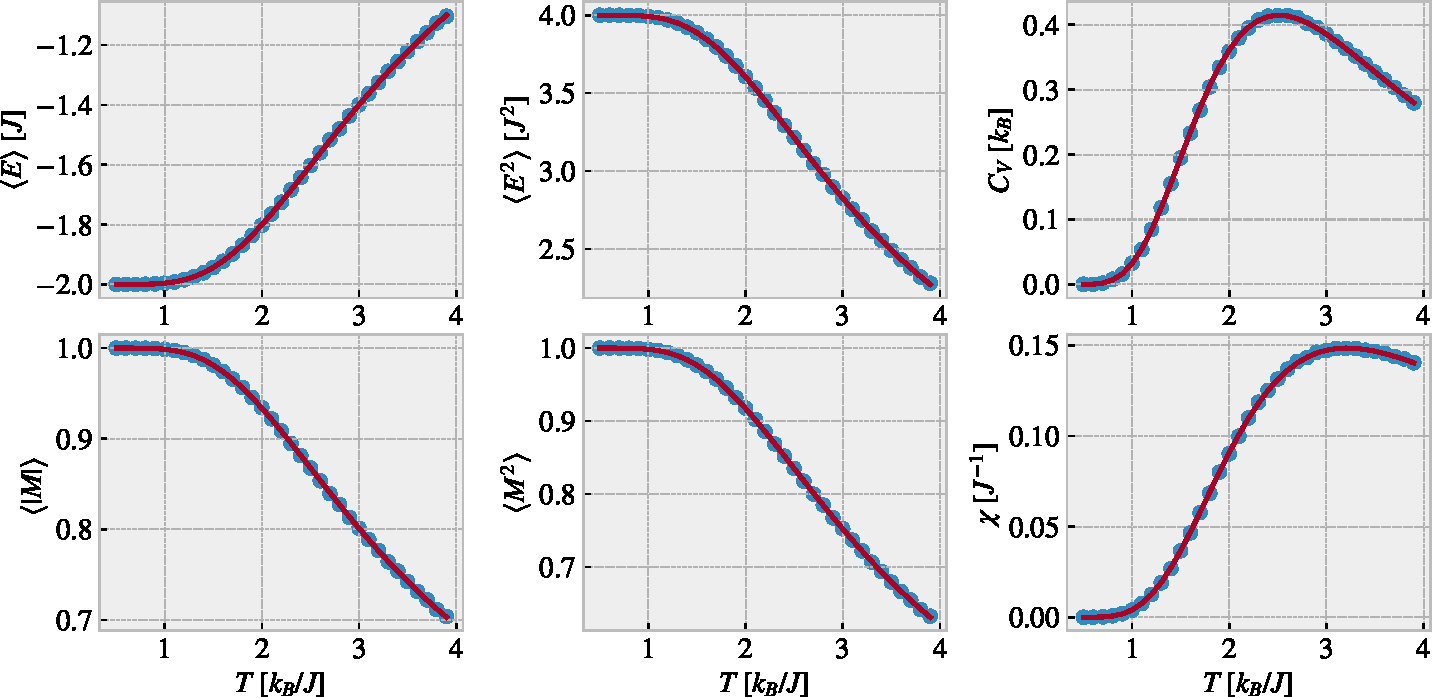
\includegraphics[width=\textwidth]{../figures/taskb.pdf}
\caption{Numerical (blue dots) and theoretical (red line) computations of the expectation value of the energy, energy squared, absolute value of the magnetization and magnetization squared as well as the heat capacity and susceptibility for a $2\times 2$ lattice as functions of temperature. This was calculated using $10^6$ MC cycles and no equilibration.}
\label{fig:taskb}
\end{figure*}


\subsection{Equilibration}

The results of the runs for $T = 1.0J/k_B$ and $T = 2.4J/k_B$ for $L = 20$ with different initial states are given in Figs. \ref{fig:L20E} (energy as function of MC cycles) and \vref{fig:L20M} (magnetization as function of MC cycles). For $T = 1.0J/k_B$, equilibrium is reached instantaneously by choosing the ordered initial state. The unordered initial state needs $\sim 10^5$ MC cycles to equilibrate. For $T = 2.4J/k_B$ both the ordered and unordered initial state reaches equilibrium after $\sim 10^4$ MC cycles. This is the reason for why we have chosen to equilibrate for $10^5$ cycles for the beginning temperatures and $10^4$ cycles for the following.


\begin{figure}
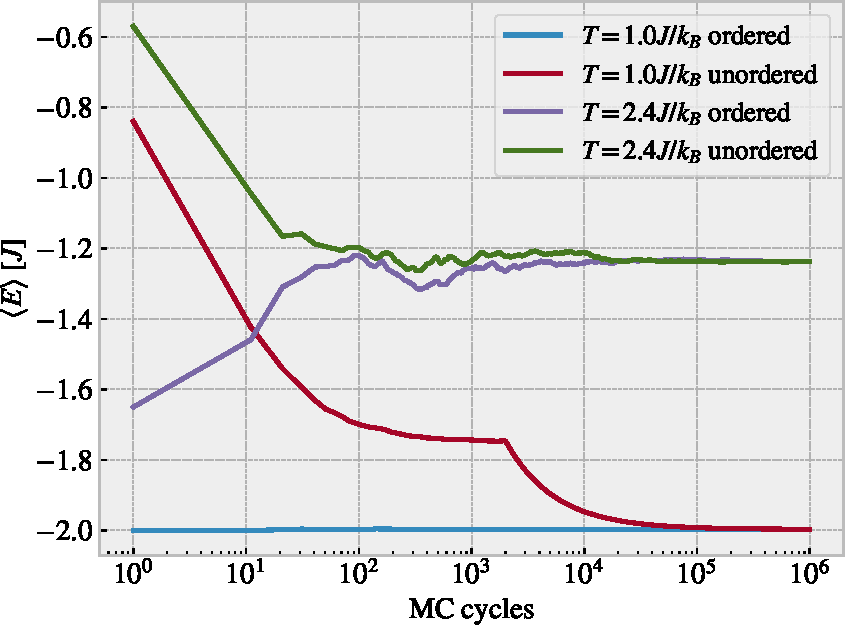
\includegraphics[width=0.485\textwidth]{../figures/problem_c_E.pdf}
\caption{The expectation value of the energy as a function of MC cycles for a $20 \times 20$ lattice. The simulation have been done for two different temperatures with two different initial configurations; ordered and unordered/disordered. Ordered means that all spins starts pointing up ($S^z = 1$), while the disordered configuration is chosen randomly.}
\label{fig:L20E}
\end{figure}



\begin{figure}
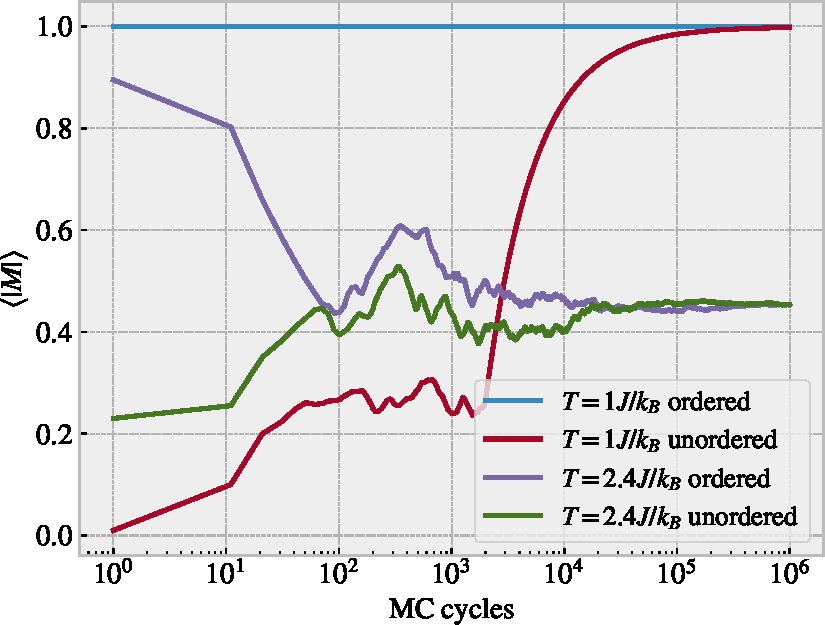
\includegraphics[width=0.485\textwidth]{../figures/problem_c_M.pdf}
\caption{The expectation value of the absolute value of the magnetization as a function of MC cycles for a $20 \times 20$ lattice. The simulation have been done for two different temperatures with two different initial configurations; ordered and unordered/disordered. Ordered means that all spins starts pointing up ($S^z = 1$), while the disordered configuration is chosen randomly.}
\label{fig:L20M}
\end{figure}

\begin{figure}
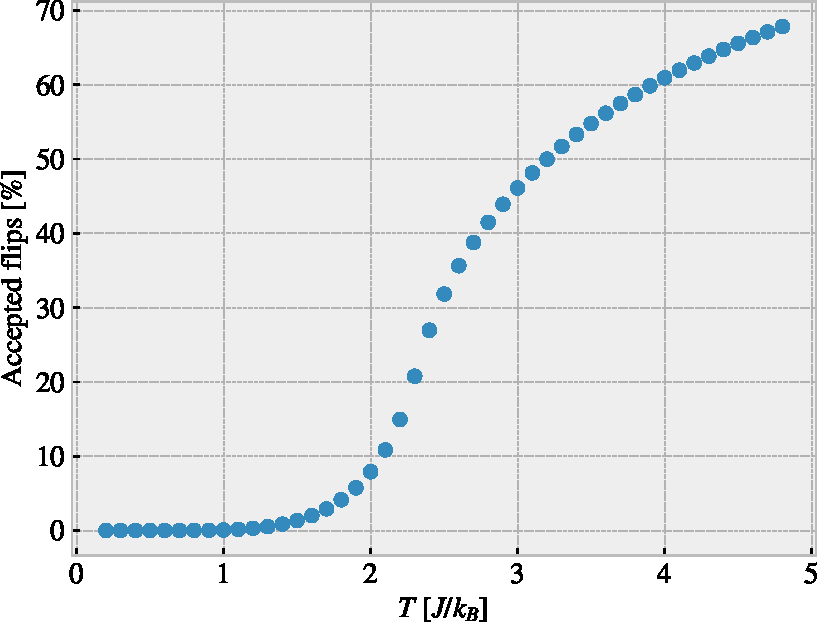
\includegraphics[width=0.485\textwidth]{../figures/problem_c_2.pdf}
\caption{The percentage of accepted states for different temperatures, calculated with a lattice size $L = 20$. We see that the percentage is low for temperatures below the critical temperature, and increasing rapidly at the critical temperature. For temperatures above the critical temperature it increases slower.}
\label{fig:L20accepting}
\end{figure}


Fig. \vref{fig:L20accepting} shows the percentage of accepted moves in the MC simulation as a function of temperature for an $L = 20$ lattice size. It is low for low temperatures and rises drastically around the analytical value for the critical temperature. It then keeps growing when increasing the temperature.

\subsection{Energy distribution}
\begin{figure}
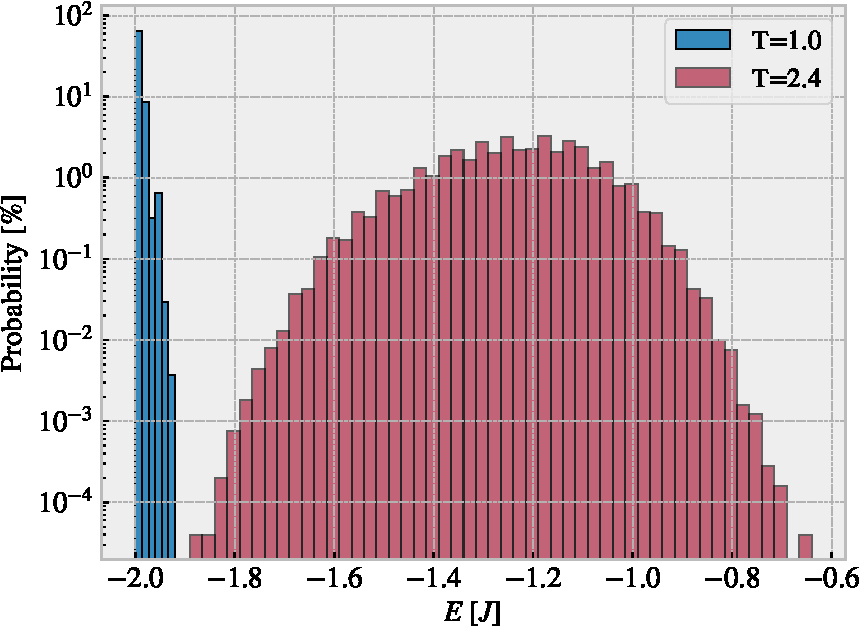
\includegraphics[width=0.485\textwidth]{../figures/problem_d.pdf}
\caption{Histograms over the energies that occurs in the system during the MC simulations for $T = 1.0J/k_B$ (blue) and $T = 2.4J/k_B$ (red). This is done for a lattice size $L = 20$ with $10^6$ MC cycles. The histograms are made with 5 bins for $T = 1.0J/k_B$ and 50 bins for $T = 2.4J/k_B$. Note that the y-axis is logarithmic.}
\label{fig:P(E)}
\end{figure}

In Fig. \vref{fig:P(E)} we show two histograms showing counts of the number of times the spin configurations ($L = 20$) have certain energies for $T = 1.0J/k_B$ (blue) and $T = 2.4J/k_B$ (red) over $10^6$ MC cycles. The histogram corresponds to the energy distributions $P(E)$ for the different temperatures. We find that the average energy is $-2.00J$ with a variance $0.01J$ for $T = 1.0J/k_B$ and $-1.25J$ with a variance $0.14J$ for $T = 2.4J/k_B$.


\subsection{Parallelization}

\begin{figure}
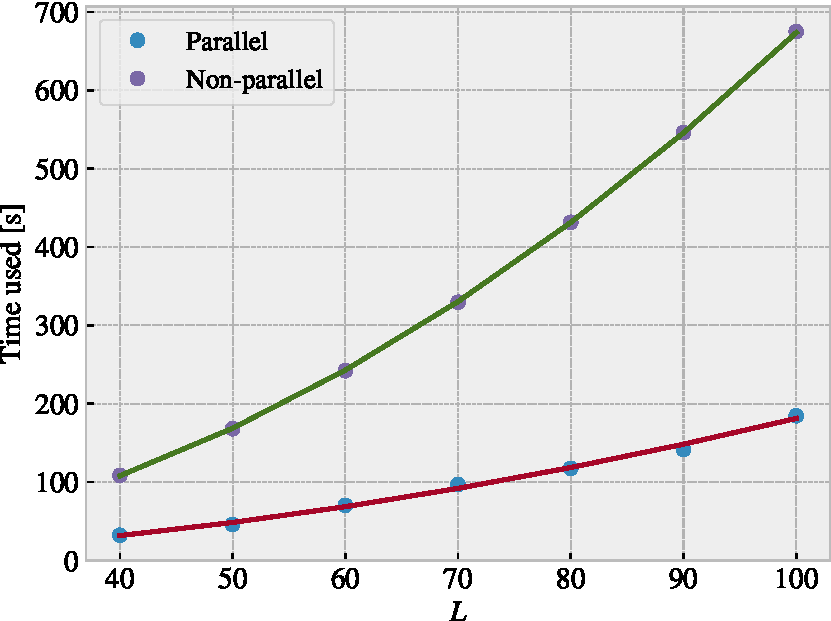
\includegraphics[width=0.485\textwidth]{../figures/timer.pdf}
\caption{The run time used by the algorithm for $105$ MC cycles and eight different temperatures as function of the lattice size $L$ for both the parallelized and unparallelized case. Four CPUs were used for the parallelization. The measured times are shown as dots, and the curves show the best fit found by the method of least squares \cite{squires}.}
\label{fig:timer}
\end{figure}

When parallelizing the code and running it on four CPUs, we get that the runtime goes as shown in Fig. \vref{fig:timer}, where we also have plotted the run time of the unparallelized code. Both are plotted as functions of the lattice size $L$, and in all cases, we ran $10^5$ MC cycles for eight different temperatures. By studying the same data in a log-log plot we find that the unparallelized code has a slope of $1.996(4)$, and the parallelized code has a slope of $1.90(5)$. When calculating the relationship of the two, we find that the parallelized code runs $3.6(2)$ times faster than the unparallelized code.

\subsection{The phase transition}

\begin{figure}
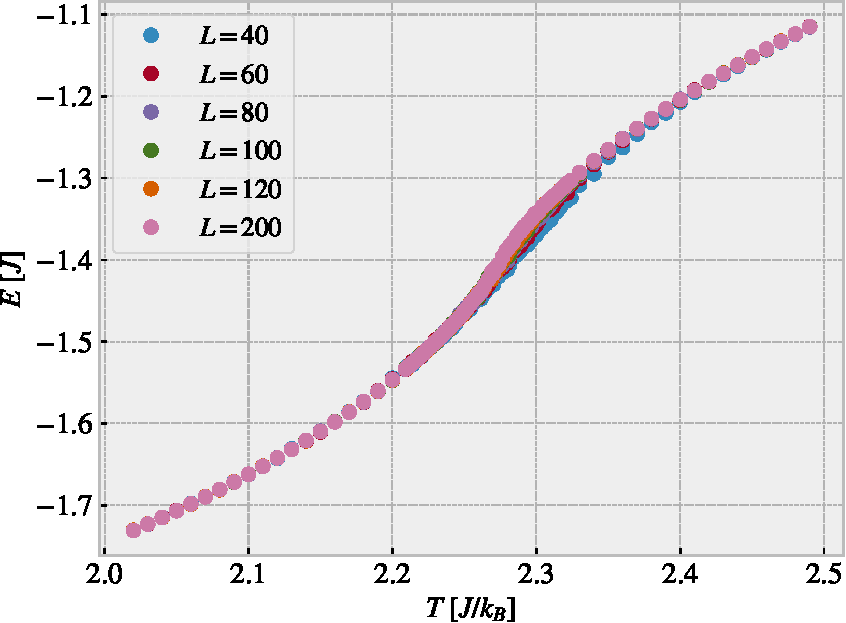
\includegraphics[width=0.485\textwidth]{../figures/energy.pdf}
\caption{The plot shows the energy per spin as a function of temperature for five different lattice sizes; $L = 40, 60, 80, 100, 120, 200$.}
\label{fig:energy}
\end{figure}

\begin{figure}
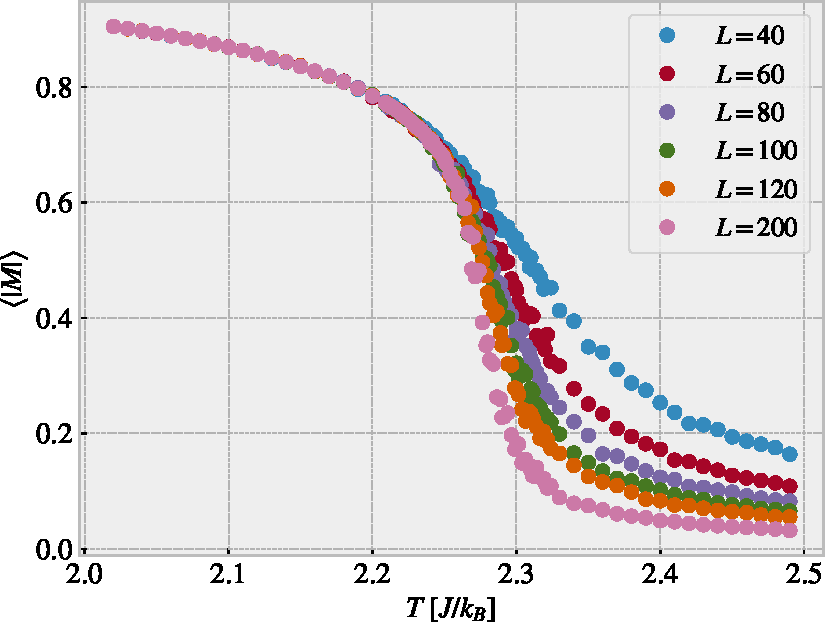
\includegraphics[width=0.485\textwidth]{../figures/magne.pdf}
\caption{The plot shows the absolute value of the magnetization per spin as a function of temperature for five different lattice sizes; $L = 40, 60, 80, 100, 120, 200$.}
\label{fig:magne}
\end{figure}

\begin{figure}
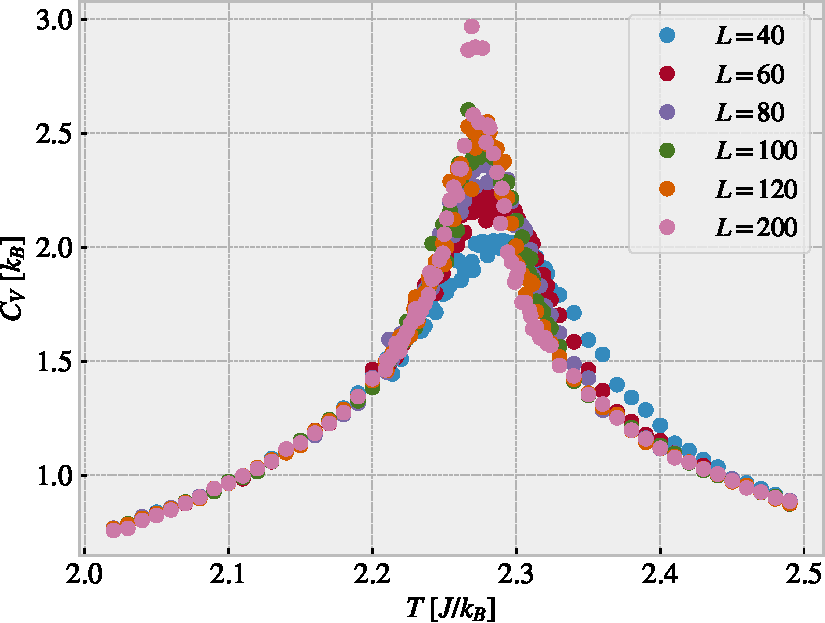
\includegraphics[width=0.485\textwidth]{../figures/heatcap.pdf}
\caption{The heat capacity per spin as a function of temperature for five different lattice sizes; $L = 40, 60, 80, 100, 120, 200$.}
\label{fig:heatcap}
\end{figure}

\begin{figure}
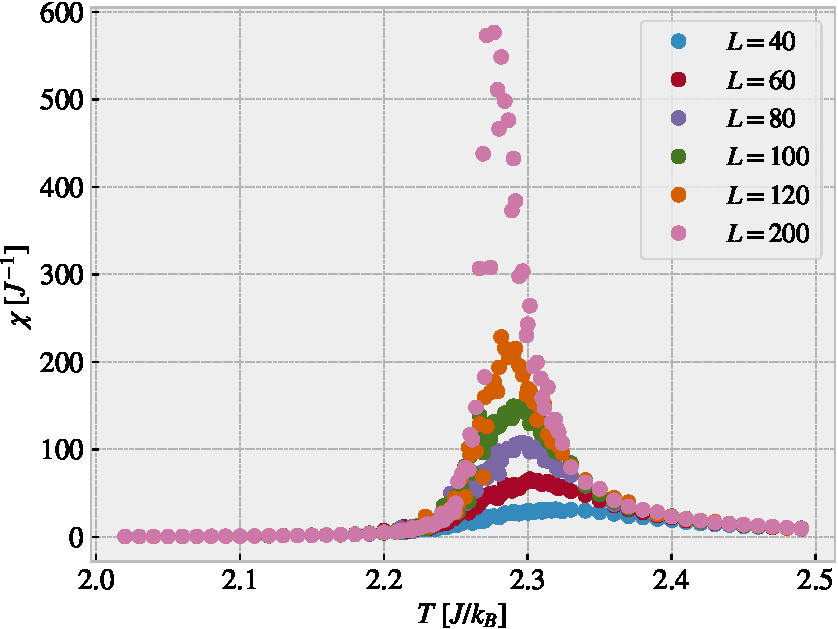
\includegraphics[width=0.485\textwidth]{../figures/suscept.pdf}
\caption{The susceptibility per spin as a function of temperature for five different lattice sizes; $L = 40, 60, 80, 100, 120, 200$.}
\label{fig:suscept}
\end{figure}

The Figs. \ref{fig:energy} - \ref{fig:suscept} shows the mean energy, mean magnetization, heat capacity and susceptibility of the system, respectively, as functions of temperature for different lattice sizes. All runs are done with $10^6$ MC cycles and an equilibration time of $10^5$ MC cycles for the first temperature in a run and $10^4$ MC cycles for the following temperatures.


By applying a Savitzky-Golay filter to the heat capacity curves, we get the curves shown in Fig. \vref{fig:fitted}. These curves were used to approximate the critical temperature at different lattice sizes. We simply said that the temperature corresponding to the maxima in the heat capacity was the critical temperature. This gave us the temperatures plotted as blue dots in Fig. \vref{fig:TC}. In this figure, we have used a linear regression \citep{squires} on the data points to find the best linear fit. According to Eq. \eqref{eq:TCinfty}, the intercept with the temperature axis should then be the critical temperature at $L\to\infty$. We find that
\begin{equation}
T_C(L\to\infty) = 2.2698(6) J/k_B.
\end{equation}


\begin{figure}
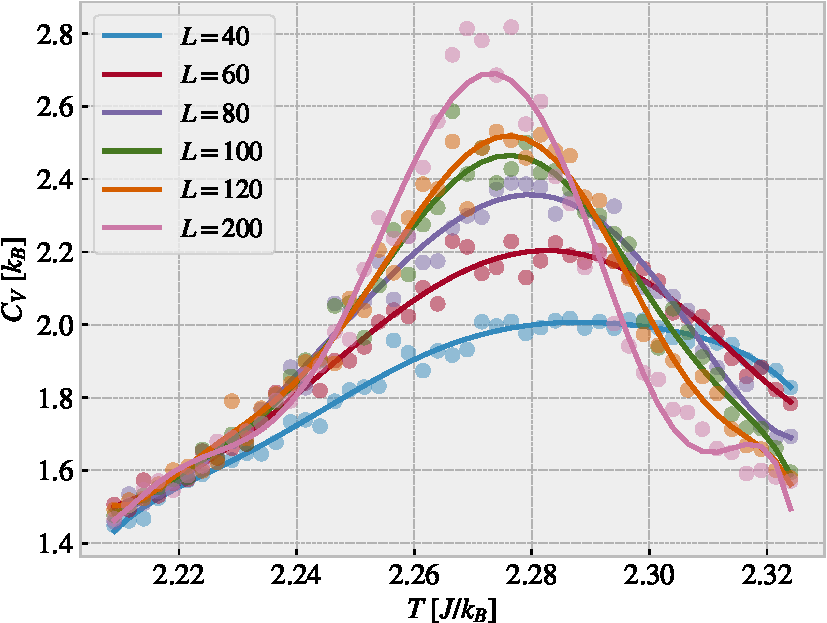
\includegraphics[width=0.485\textwidth]{../figures/fitted_suscept.pdf}
\caption{The heat capacities found by MC simulations using $10^6$ MC cycles are shown as dots for $L = 40, 60, 80, 100, 120, 200$. The filtered curves, found by using a Savitzky-Golay filter, are plotted with colours corresponding to the dots.}
\label{fig:fitted}
\end{figure}


\begin{figure}
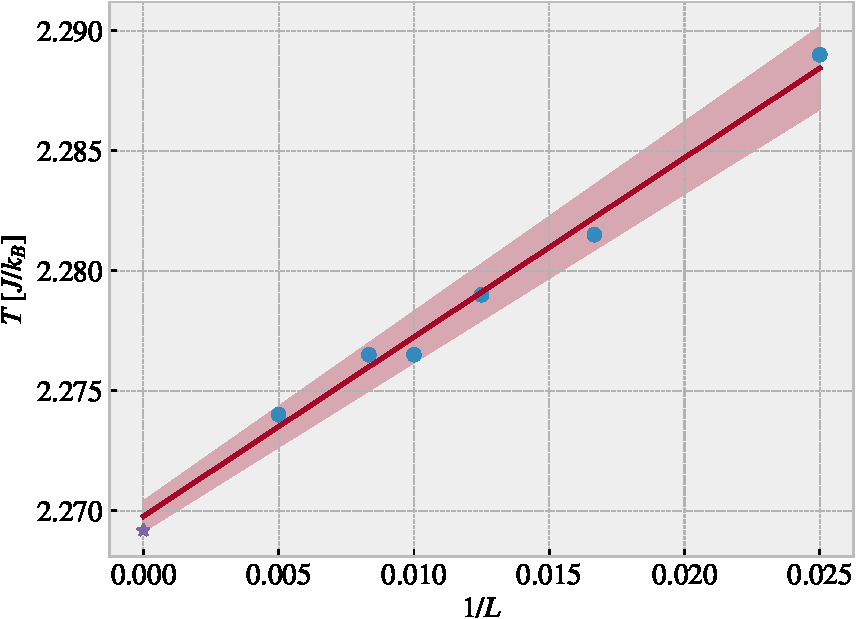
\includegraphics[width=0.485\textwidth]{../figures/TC.pdf}
\caption{The dots mark the temperatures where the heat capacity peaks (after we applied the Savitzky-Golay filter) for different lattice sizes $L = 40, 60, 80, 100, 120, 200$, which is interpreted as the critical temperature of the system. This is plotted against $1/L$. Using a linear regression \cite{squires} on this data, the critical temperature at $L \to \infty$ can be interpreted as the constant term, which is $T_C(L\to\infty) = 2.2698 \pm  0.0006 J/k_B$. The star shows the analytical value for the critical temperature $T_C = 2.2692J/k_B$ \citep{onsager}.}
\label{fig:TC}
\end{figure}


\begin{figure*}
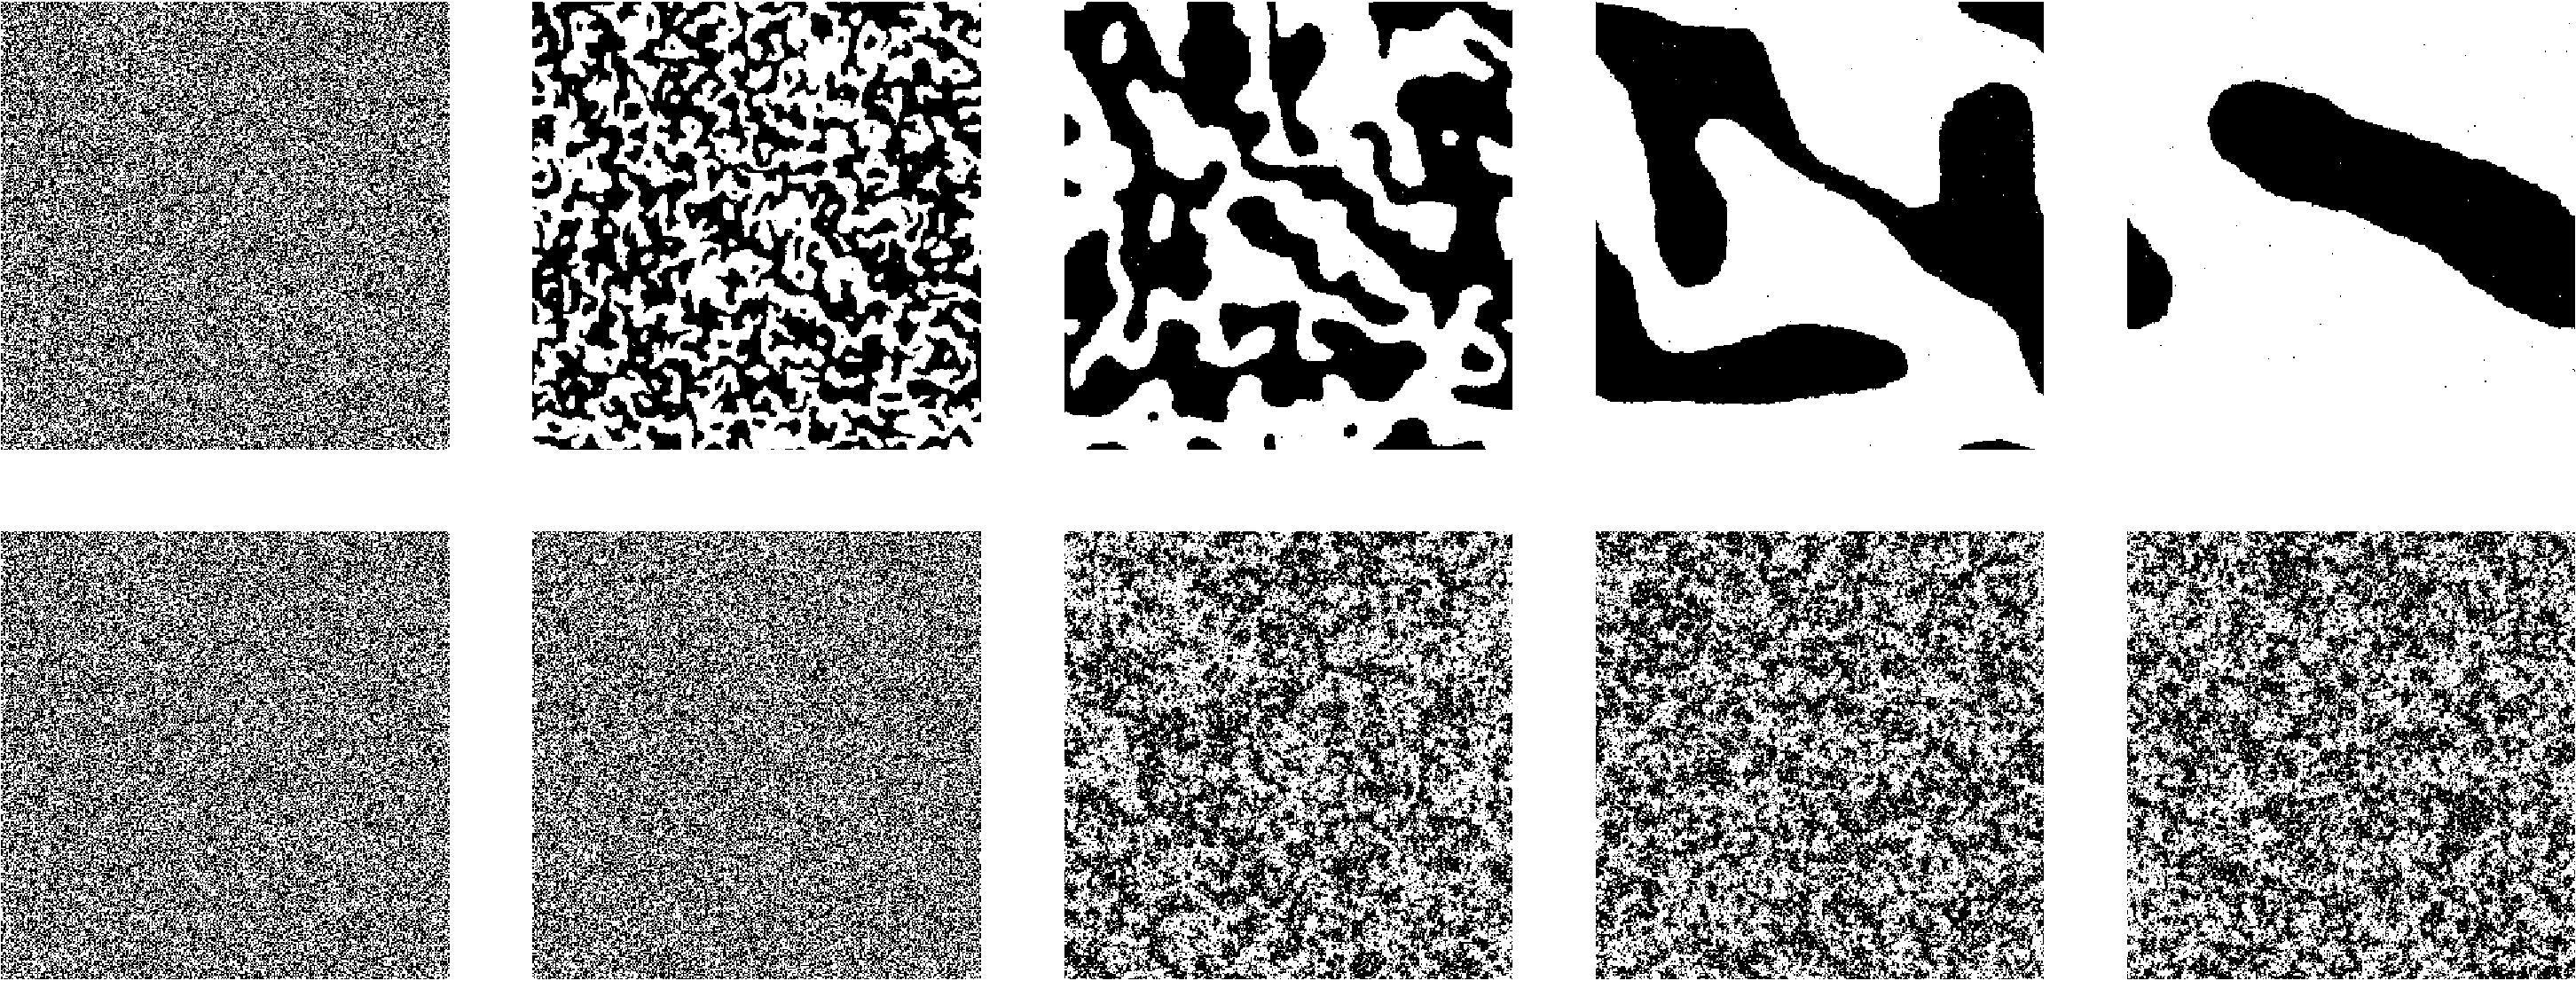
\includegraphics[width=\textwidth]{../figures/evolution.pdf}
\caption{The figure shows the evolution of the spin configuration for a $L = 1000$ lattice. Black represents a spin pointing down, white represents a spin pointing up. The top row shows the evolution for $T = 1.0J/k_B$, the bottom row shows the evolution  for $T = 2.4J/k_B$. The columns from left to right show the configurations after $0$, $10^2$, $10^3$, $10^4$ and $10^5$ MC cycles. Both systems started out in a random initial state.}
\label{fig:evolution}
\end{figure*}

Fig. \vref{fig:evolution} shows the evolution of the spin configurations at different points in time (different MC cycle numbers). The top row has $T = 1.0J/k_B$, while the bottom row has $T = 2.4J/k_B$. In both cases, we have used $L = 1000$. In this figure, black represents a spin pointing down and white represents a spin pointing up.


\section{Discussion}

\subsection{Benchmarking}
From Fig. \vref{fig:taskb}, we see that the algorithm reproduce the analytical results of Eq. \eqref{eq:expvals} - \eqref{eq:suscept}. Thus, we have good reasons to expect that our algorithm is implemented correctly, and that it will produce correct results also for bigger lattice sizes. Thus, this shows that we with high probability can count on the results produced by the MC simulations when studying the phase transition. What is more questionable is the choice of equilibration time.


\subsection{Equilibration}

Figs. \ref{fig:L20E} and \vref{fig:L20M} show that how fast equilibrium is reached depends on the initial state for low temperatures, but is unaffected of initial state for the higher temperature. This can easily be explained. For low temperatures, i.e. temperatures below the critical temperatures, an ordered state is favoured. We are in the ferromagnetic phase of the system. If the temperature is low enough, one would even expect a pure ferromagnet, where all the spins point in the same direction. Therefore, when starting in an ordered state for low temperatures, this is already the steady state for $T = 1.0J/k_B$, and equilibrium is reached instantaneously. We stay in the steady state because of the Metropolis accepting rule, which  give a very small probability of flipping a spin when in steady state. And if a spin gets flipped, it is probable that it will be flipped back again. 

When starting in an unordered state on the other hand almost all flips get accepted in the start, as we are far from steady state. We see that for $T = 1.0J/k_B$, the configuration converges towards an almost steady state (analogous to another eigenvalue of the transition matrix, when considering Markov chains), then suddenly a flipping do so that a more likely state is found, and the solution converges towards the real equilibrium. In total the whole process takes $10^4-10^5$ MC cycles.

For the higher temperature $T = 2.4J/k_B$, we see that the equilibration time is independent on whether the initial state is ordered or not. In this case we expect an almost non-magnetized configuration, that should be $50\%$ of the spins pointing up, and the rest pointing down. We see though from Fig. \vref{fig:L20M} that the magnetization is non-zero for the steady state. This follows from the small lattice size. For this lattice size, the critical temperature is still above $2.4J/k_B$. Thus, we do not expect an completely unordered state. The spins are still somewhat correlated, and we are still in the ferromagnetic phase. This explains why neither the ordered nor the unordered configuration is the steady state, and both reach the steady state equally fast $\sim 10^5$ MC cycles. For temperatures above the critical temperature, we expect the unordered configuration to be closer to the steady state. 

These results are the reason for why we chose $10^5$ MC cycles as the initial equilibration time and $10^4$ for the following, as the following start out in a state close to the steady state, while the initial run start out in a random configuration. We make a guess that this will hold also for bigger systems, as the number of flipped spins in each MC cycle also increase. This method is much simpler to implement, and saves a lot of CPU time, compared to a method that check frequently whether equilibrium is reached or not.


Fig. \vref{fig:L20accepting} shows the number of accepted flips during $10^5$ MC cycles plotted against temperature. We see that, as expected, few proposed flips are accepted below the critical temperature, where we are in the ferromagnetic phase. This is because the spins are correlated. Thus, when the steady state is reached, no (or very few) flips are accepted. Therefore the total percentage of accepted flips is almost zero. As we approach the critical temperature, the percentage starts to increase. This is because the thermal fluctuations are starting to be noticeable.

At high temperatures the percentage of accepted states are high, more than $50\%$. This is because the state is unordered, and thus we can continue flipping spins without changing the energy much, as the spins are almost uncorrelated. Thus there are many states minimizing the free energy. One would expect the curve of accepted states to approach $100\%$ for high enough temperatures, as the system is completely governed by the thermal fluctuations, so that the magnetic interactions are negligible.


\subsection{Energy distribution}

The energy distribution shown in Fig. \vref{fig:P(E)} shows that the mean energy is low for low temperatures and higher for higher temperatures, as expected. We also see that the variance is bigger at higher temperatures. This is also natural, as the thermal fluctuations also increase, and the spins become more uncorrelated, thus the spin configuration have less impact on the total free energy, which we would like to minimize, and a high entropy state is favoured.

An advantage of the Monte Carlo simulations is that we can get this probability distribution function without actually calculating it. Calculating it that would have included calculating the partition function, which is out of question for big systems. 


\subsection{Parallelization}

When running on four CPUs, we found that the run time was $3.6(2)$ times faster than without parallelization. This is less than $4$, which would have been the optimal value, but it is not far from $4$. The unparallelized code goes as $L^{1.996(4)}$ and the parallelized code goes as $L^{1.90(5)}$, so they scale almost the same with $L$ and almost as $L^2$, which is what we would have expected. The reason why they don't go as $L^2$ is e.g. that there are other processes in the programs that are independent of $L$. There are more of such processes in the case of parallelized code, as the machine have to distribute the work on the different CPUs. This may explain why the power of $L$ is less in the parallelized case.


\subsection{The phase transition}
Fig. \vref{fig:energy} shows that the energy increases as the temperature increases. This is expected, as the spin configuration becomes more disordered. We also see that the energy increases faster around the critical temperature for bigger lattices, which can be explained by Fig. \vref{fig:heatcap}. The heat capacity measures the change in energy per temperature, and we see that this is bigger for large lattices around the critical temperature.

We think that Fig. \vref{fig:magne} show some good results. This is the magnetic order parameter, which is expected to be non-zero below the critical temperature and zero above the critical temperature. This graph shows us that the critical temperature gets closer and closer to the analytical value as the lattice size increases. We also see that the phase transition become more well-defined, in the sense that one would expect the slope of the order parameter to approach infinity at the critical temperature. The continuity of the magnetization at the critical temperature indicates a continuous phase transition \cite{blundell}, which is what we expect for the paramagnetic to ferromagnetic phase transition in a 2D Ising model on a square lattice.

Both the heat capacity (Fig. \vref{fig:heatcap}) and susceptibility (Fig. \vref{fig:suscept}) peaks around the critical temperatures, as expected from Eqs. (18) - (19). We interpret the temperature corresponding to the peak of the heat capacity as the critical temperature of the system of a given lattice size. Fig. \vref{fig:fitted} gave us the critical temperatures for $L = 40, 60, 80, 100, 120, 200$. Thiese results could maybe be bettered by using another degree of the polynomials or another number of coefficients, but the values we chose were chosen so that the graphs become as smooth as possible around the peaks, which also gave the most linear relation, shown in Fig. \vref{fig:TC}. Thus, we ended up with $T_C(L\to\infty) = 2.298(6)J/k_B$, which first of all has a high precision, and the accuracy is not too bad either. Our result is corresponding to the analytical result of Onsager within the uncertainties. 

One could ask why we chose to use the heat capacity and not the susceptibility to estimate the critical temperature. This is because we believe the uncertainties in energy to be less than those in magnetization. This is based on Figs. \ref{fig:L20E} and \vref{fig:L20M}, where we see that the magnetization fluctuates more than the energy also after equilibration. 

The results could be bettered by using more MC cycles and bigger lattices. Also, we could consider using a more accurate method of equilibration, but as the calculations were already quite long, we chose to use the method of equilibration that used least time. If time had allowed for it, it would be a good idea to check more closely whether the equilibration time is enough for our lattice sizes.

Fig. \vref{fig:evolution} shows the difference in the configurations above and below the critical temperature. We clearly see more clustering of aligned spins for $T = 1.0J/k_B$ compared to $T = 2.4J/k_B$, and it looks like the majority of the spins are pointing up (white). We see that the system with $T = 1.0J/k_B$ starts out in an unordered configuration, but after only $10^2$ MC cycles, we see tendencies of clustering. This gets more and more visible, and at $10^5$ There is only one region where spins points down. By further decreasing the temperature from $1.0J/k_B$, we would expect the white parts to outperform the black, ending up all spins pointing up.  For $T = 2.4J/k_B$ there is approximately an even distribution of spins pointing up and down through the whole simulation (no net magnetization, paramagnetic phase). These results fit well with theory. $T = 1.0J/k_B$ is below the critical temperature, and as Fig. \ref{fig:evolution} shows, we get clusters of ordered spins for this temperature, as expected in a ferromagnetic phase. For $T = 2.4J/k_B$ theory tells us that as we are above the critical temperature, we should be in an paramagnetic phase, which is also what we observe; The spins are disordered. 


\section{Conclusion}

We have studied phase transitions in a two dimensional Ising ferromagnet on a square lattice. The critical temperature was found by doing Monte Carlo simulations with the Metropolis algorithm as accepting rule. By calculating the heat capacity for different lattice sizes, we could extract the critical temperature by locating the maximum of the heat capacity. To reduce the effect of fluctuations in the results, we applied a Savitzky-Golay filter. Linear regression of the critical temperatures as functions of $1/L$ then gave us a critical temperature for an infinite lattice
\begin{equation}
T_C(L\to\infty) = 2.2698(6)J/k_B,
\end{equation}
which agrees with the analytical solution of L. Onsager \cite{onsager} within the uncertainties.

We believe that our results are trustworthy from benchmarking with a $2 \times 2$ lattice, and also from the good agreement with theory for $T_C(L\to\infty)$. 

We also saw the benefit of parallelization when doing MC simulations, as we reduced the run time by a factor of $3.6(2)$ by parallelizing 4 CPUs. 



\section{Comments}
All of the code used is available on our GitHub\footnote{\url{http://www.github.uio.no/cecilgl/FYS4150}}. Here the \texttt{README.MD} files will describe the structure of our GitHub, and what each program was used for. The code itself will also include notes explaining what we do.



\begin{thebibliography}{99}
\bibitem{onsager} L. Onsager, Phys. Rev. \textbf{65}, 117 (1944).
\bibitem{hjorten} M. Hjorth-Jensen, Computational Physics Lecture Notes Fall 2015 (2015).
\bibitem{flekkoy} F. Ravndal and E.G. Flekkøy, Statistical Physics - a second course (2014).
\bibitem{squires} G.L. Squires, Practical Physics, Cambridge University Press (2001).
\bibitem{blundell} S. Blundell, Magnetism in Condensed Matter, Oxford University Press (2001).
\end{thebibliography}


\end{document}
%
% ****** End of file apssamp.tex ******
